%\tableofcontents
\chapter{Nonequilibrium-induced Lifshitz transitions}
\label{chap:FS}

\section{Introduction}
In this chapter, we introduce time-dependent light-induced engineering of the Fermi surface (FS) for materials with strong electronic correlations. 

An external electric field changes the band structure \cite{Principi_2016}, and as a result a change in the FS occurs. Such an electronic topological transition called Lifshitz transition.
We address nonequilibrium-induced Lifshitz transition caused by the applied external electric field in a case one-band Hubbard model on a 2D square lattice.

The Lifshitz transition can be also induced by doping, external pressure or external magnetic field and has been experimentally observed in many real systems, such as heavy-fermion systems 
\cite{PhysRevB.86.075108, PhysRevLett.110.256403, PhysRevLett.116.037202}, 
iron-based superconductors \cite{PhysRevB.83.020501, PhysRevB.86.165117, PhysRevB.88.220508, PhysRevLett.112.156401, PhysRevB.90.224508, Liu_2010_FS}, 
cuprate high-temperature superconductors \cite{PhysRevB.81.180513, PhysRevB.83.054506, PhysRevLett.114.147001, PhysRevLett.120.067002, PhysRevB.81.121102}.


%\FloatBarrier


%\section{\label{Theory} Model and method}

We take the single-band Hubbard model driven by an electric field with the Hamiltonian:
\begin{equation}
\begin{split}
H(t)&=\sum_{ij,\sigma}t_{ij}{\rm exp}{\left( -i\int_{{\bf R}_{j}}^{{\bf R}_{i}}d{\bf r} \cdot {\bf A}(t) \right)}c_{i \sigma}^{\dagger}c_{j \sigma}\\
&+\mu {\sum_{i,\sigma} n_{i \sigma}}+U{\sum_{i} n_{i \uparrow}n_{i \downarrow}},
\end{split}
\end{equation}
where $t_{ij}$ is electron hopping amplitudes between sites $i$ and $j$, $U$ is the on-site Coulomb interaction, $c_{i \sigma}^{\dagger}$ creates an electron at site $i$ and spin $\sigma$, and 
$n_{i\sigma}=c_{i\sigma}^{\dagger}c_{i\sigma}$ is the number operator. We incorporate the effect of 
an external electric field ${\bf E(t)} = -\partial{\bf A}(t)/\partial t$ in terms of the Peierls
substitution \cite{Peierls1933} for the vector potential ${\bf A}$ into the hopping \cite{PhysRevLett.106.236401, PhysRevB.91.245153}.  

Exploiting this property, we can direct the electric field along one of the crystallographic axes, which gives a quasi-one-dimensional model, 
or along the diagonal of the square lattice, which gives physics similar to the hypercubic lattices but with the 2D band structure that includes the van Hove singularity.

In order to treat the time-dependent problem, we use non-equilibrium IPT which was discussed in Sec. \ref{subsection:Impurity_solvers} of \autoref{chap:Non_mb_th} in detail.

We consider the square lattice with the band dispersion,
\begin{equation}
\begin{split}
 \varepsilon({\bf k},t)&=2t\left[{\rm cos}(k_x+A_x(t))+
{\rm cos}(k_y+A_y(t))\right]\\
 &+4t'{\rm cos}(k_x+A_x(t)) {\rm cos}(k_y+A_y(t)),
 %\\
 % &{ { +2t_3(cos(2k_x+2{\bf A}_x(t))+cos(2k_y+2{\bf A}_y(t)))}}.
\end{split}
\label{dispersion}
\end{equation}
where $t=1$ is the nearest-neighbor (NN) and $t'=-0.32$ is next nearest-neighbor (NNN) hopping amplitude. 
Time has units of reverse hoppings. 
DMFT based retarded and lesser Green's functions can give information about excitation and occupation spectrum Eq. \eqref{Spectr_R_L_1},\eqref{Spectr_R_L_2} in Sec. \ref{subsection:Spectral_function} of \autoref{chap:Non_mb_th}. The $k$-resolved spectral function and occupied density of states diven by Eq. \eqref{Spectr_R_L_k_1},\eqref{Spectr_R_L_k_2} in Sec. \ref{subsection:Spectral_function} of \autoref{chap:Non_mb_th}.
The shape of the vector potential is depicted in Fig.~\ref{fig:A_shape_FS}.
\begin{figure}[h!]
%\begin{minipage}[h]{0.51\linewidth}
\center{\includegraphics[width=0.6\linewidth]{Chapters/Fermi_surface/figures/Pulse_shape.eps}} \\
%\end{minipage}
\caption{Shape of vector potential ($\omega=21$, $t_0=6.85$).}
\label{fig:A_shape_FS}
\end{figure}
and is expressed by the formula:
\begin{equation}
%A(t)={A_{\rm max}{\rm exp}\left[-\frac{(t-t_0)}{2\sigma ^2}]}sin[\omega(t-t_0)+\phi+\frac{r_c t^2}{2}\right],
A(t)={A_{\rm max}{\rm exp}\left[-\frac{(t-t_0)^2}{2\sigma ^2}\right]}sin(\omega(t-t_0)),
\label{Ashape}
\end{equation}
where parameters are:
$\sigma=\frac{d}{2\sqrt{2ln2}}$; pulse duration with $d$; full-width at half-maximum (FWHM);
amplitude of the vector potential $A_{\rm max}$;
frequency of the vector potential $\omega$;
peak time of the pulse $t_0$.
Below we provide calculations for $\beta=5$ and $32 \times 32$ $k$-grid. 

%%%%%%%%%%%%%%%%%%%%%%%%%%%%%%%%%%%%%%%%%%%%%%%%%%%%%%%%%%%%%%%%%%
\FloatBarrier

\section{Case of the NN-hopping}

\subsection{FS parameters selection}

Calculating the FS we have to move from $k$-independent local quantities to $k$-resolved. In the first part of the chapter, we consider a square lattice with the nearest neighbors hopping whose FS is represented by a dashed line in the Fig.~\ref{fig:BZ_sq_lat}.
\begin{figure}[h!]
%\begin{minipage}[h]{0.51\linewidth}
\center{\includegraphics[width=0.35\linewidth]{Chapters/Fermi_surface/figures/square_lattice/BZ_1.pdf}} \\
%\end{minipage}
\caption{Brillouin zone for a square lattice}
\label{fig:BZ_sq_lat}
\end{figure}
Using the Green's functions on the Keldysh contour for a finite-dimensional lattice is computationally expensive and heavily limits the time of the simulations. In this chapter, we focus on transient dynamics and states immediately after the pulse. 
\begin{figure}[h!]
\begin{minipage}[h]{0.5\linewidth}
\center{\includegraphics[width=1\linewidth]{Chapters/Fermi_surface/figures/square_lattice/xy/G_l_loc.png}} (a) \\
\end{minipage}
\hfill
\begin{minipage}[h]{0.5\linewidth}
\center{\includegraphics[width=1\linewidth]{Chapters/Fermi_surface/figures/square_lattice/y/1_75/G_l_loc.png}} (b) \\
\end{minipage}
\caption{Local $G^{<}(t,t')$ for $A_{max}=1.75$ and $U=6$ with different polarizations of vector potential: (a) $XY$- polarization; (b) $Y$-polarization.}
\label{fig:G_loc_3d}
\end{figure}
Also, we define the model parameters to be the most suitable for the FS interpretation.

In the presence of a particle-hole symmetry, the challenge is to achieve a decay of the Green's functions inside considered simulation time.
In the case of local Green's functions, the damping occurs rather quickly for all considered polarizations of the external field (Fig.~\ref{fig:G_loc_3d}). Such attenuation in time will give a quantitatively correct result for the frequency dependence quantities obtained via Fourier transform. 
\begin{figure}[h!]
\begin{minipage}[h]{0.5\linewidth}
\center{\includegraphics[width=1\linewidth]{Chapters/Fermi_surface/figures/square_lattice/Gret_xy_mid_Y_u.eps}} (a) \\
\end{minipage}
\hfill
\begin{minipage}[h]{0.5\linewidth}
\center{\includegraphics[width=1\linewidth]{Chapters/Fermi_surface/figures/square_lattice/Gret_xy_mid_M_2_u.eps}} (b) \\
\end{minipage}
\caption{$G^{R}(t,t-s)_k$ ($time=6.85$) with different $U$ values for $A_{max}=1.5$ and $XY$-polarization: (a) Y-point of BZ; (b) M/2-point of BZ.}
\label{fig:G_k_res_ret_u_dep}
\end{figure}

In the case of $k$-resolved Green's functions, the damping is much slower for particular $k$-points. In Fig.~\ref{fig:G_k_res_ret_u_dep} the dependence of the Green's function on time for different $U$ is shown for Y and M/2-points in the Brillouin zone (BZ). 
\begin{figure}[h!]
\begin{minipage}[h]{0.5\linewidth}
\center{\includegraphics[width=1\linewidth]{Chapters/Fermi_surface/figures/square_lattice/Gret_xy_mid_Y.eps}} (a) \\
\end{minipage}
\hfill
\begin{minipage}[h]{0.5\linewidth}
\center{\includegraphics[width=1\linewidth]{Chapters/Fermi_surface/figures/square_lattice/Gret_xy_mid_M_2.eps}} (b) \\
\end{minipage}
\caption{$G^{R}(t,t-s)_k$ ($time=6.85$) with different $A_{max}$ values for $U=6$ and $XY$-polarization : (a) Y-point of BZ; (b) M/2-point of BZ.}
\label{fig:G_k_res_ret_A_dep_xy}
\end{figure}
Increasing Coulomb interaction the dumping of the Green's function becomes stronger. These highly symmetrical points were chosen due to the fact that they belong to the FS and have the highest intensity of the spectral function at a frequency equal to zero and the smallest attenuation of the corresponding two-time Green's function. 

In the Fig.~\ref{fig:G_k_res_ret_A_dep_xy} the dependence of the Green's function on time for different values of vector potential for $XY$-polarization of vector potential is shown. An increase of the vector potential leads to a faster decay of the Green's function. 
\begin{figure}[ht]
\begin{minipage}[h]{0.5\linewidth}
\center{\includegraphics[width=1\linewidth]{Chapters/Fermi_surface/figures/square_lattice/DOS_xy_mid_Y.eps}} (a) \\
\end{minipage}
\hfill
\begin{minipage}[h]{0.5\linewidth}
\center{\includegraphics[width=1\linewidth]{Chapters/Fermi_surface/figures/square_lattice/OCC_xy_mid_Y.eps}} (b) \\
\end{minipage}
\caption{Spectrum of the full number of states $A^{R}(t=6.85,\omega)_{k=\text{Y}}$ (a) and occupied states $A^{<}(t=6.85,\omega)_{k=\text{Y}}$ (b) with different $A_{max}$ values for $U=6$ and $XY$-polarization.}
\label{fig:G_k_res_ret_A_dep_w_xy}
\end{figure}

The corresponding spectral functions are shown in the Fig.~\ref{fig:G_k_res_ret_A_dep_w_xy}. Some of them have negative values \citep{PhysRevB.71.085104,PhysRevB.73.209902,PhysRevB.80.115119,PhysRevLett.112.176404} that partially appear as a result of the particular form of the Fourier transform used on the work.
\begin{figure}[ht]
\begin{minipage}[h]{0.5\linewidth}
\center{\includegraphics[width=1\linewidth]{Chapters/Fermi_surface/figures/square_lattice/Gret_y_mid_Y.eps}} (a) \\
\end{minipage}
\hfill
\begin{minipage}[h]{0.5\linewidth}
\center{\includegraphics[width=1\linewidth]{Chapters/Fermi_surface/figures/square_lattice/Gret_y_mid_M_2.eps}} (b) \\
\end{minipage}
\caption{$G^{R}(t,t-s)_k$ ($time=6.85$) with different $A_{max}$ values for $U=6$ and $Y$-polarization: (a) Y-point of BZ; (b) M/2-point of BZ.}
\label{fig:G_k_res_ret_A_dep_y}
\end{figure}

As can be seen from Fig.~\ref{fig:G_k_res_ret_A_dep_y}, similar dependence of the attenuation of the Green's functions on the magnitude of the vector potential takes place for the case of $Y$-polarization.
Also, similar to the $XY$-polarization case, $Y$-polarized pulse transfers states (Fig.~\ref{fig:G_k_res_ret_A_dep_w_y}a) and particles (Fig.~\ref{fig:G_k_res_ret_A_dep_w_y}b) from the low-frequency to the high-frequency region.
\begin{figure}[h!]
\begin{minipage}[h]{0.5\linewidth}
\center{\includegraphics[width=1\linewidth]{Chapters/Fermi_surface/figures/square_lattice/DOS_y_mid_Y.eps}} (a) \\
\end{minipage}
\hfill
\begin{minipage}[h]{0.5\linewidth}
\center{\includegraphics[width=1\linewidth]{Chapters/Fermi_surface/figures/square_lattice/OCC_y_mid_Y.eps}} (b) \\
\end{minipage}
\caption{Spectra of full number of states $A^{R}(t=6.85,\omega)_{k= \text{Y}}$ (a) and occupied states $A^{<}(t=6.85,\omega)_{k= \text{Y}}$ (b) for different $A_{max}$ values with $U=6$ and $Y$-polarization.}
\label{fig:G_k_res_ret_A_dep_w_y}
\end{figure}

In order to understand how the redistribution of electrons occurs due to increasing of the magnitude and direction of the pulse, we consider the local lesser Green's functions (Fig.~\ref{fig:G_loc_les_A_dep_w}). For all pulse polarizations, the maximum pumping of the Hubbard bands occurs in the region around the maximum of the pulse ($time=6.85$) due to the transfer of electrons to higher energy regions at $U/2$.
The higher the value of the vector potential becomes stronger the intensity of the Hubbard band and less in the low-frequency region for the $Y$-the direction of the vector potential (Figs.~\ref{fig:G_loc_les_A_dep_w}b,d,f). In the case of $XY$-polarization, the electron population of the low-frequency region can oscillate depending on the renormalized hopping value in accordance with the zero-order Bessel function \cite{PhysRevLett.106.236401}. The van Hove singularity nearly disappears in the pulse maximum at the $A_{max}=3.0$ for all polarizations.
Thus, for these parameters of the system, it is prudent to use a $A_{max}=1.75$ in which the convergence of the two-time Green's function is good and at the same time, there is a high density of states at the Fermi level during the pulse.
\begin{figure}[h!]
\begin{minipage}[h]{0.5\linewidth}
\center{\includegraphics[width=1\linewidth]{Chapters/Fermi_surface/figures/square_lattice/1_5_xy.png}} (a) \\
\end{minipage}
\hfill
\begin{minipage}[h]{0.5\linewidth}
\center{\includegraphics[width=1\linewidth]{Chapters/Fermi_surface/figures/square_lattice/1_5_y.png}} (b) \\
\end{minipage}
\begin{minipage}[h]{0.5\linewidth}
\center{\includegraphics[width=1\linewidth]{Chapters/Fermi_surface/figures/square_lattice/1_75_xy.png}} (c) \\
\end{minipage}
\hfill
\begin{minipage}[h]{0.5\linewidth}
\center{\includegraphics[width=1\linewidth]{Chapters/Fermi_surface/figures/square_lattice/1_75_y.png}} (d) \\
\end{minipage}
\begin{minipage}[h]{0.5\linewidth}
\center{\includegraphics[width=1\linewidth]{Chapters/Fermi_surface/figures/square_lattice/3_0_xy.png}} (e) \\
\end{minipage}
\hfill
\begin{minipage}[h]{0.5\linewidth}
\center{\includegraphics[width=1\linewidth]{Chapters/Fermi_surface/figures/square_lattice/3_0_y.png}} (f) \\
\end{minipage}
\caption{Occupied states $A^{<}(t,\omega)$ for $U=6$: (a) $A_{max}=1.5$ $XY$-polarization; (b) $A_{max}=1.5$ $Y$-polarization; (c) $A_{max}=1.75$ $XY$-polarization; (d) $A_{max}=1.75$ $Y$-polarization; (e) $A_{max}=3.0$ $XY$-polarization; (f) $A_{max}=3.0$ $Y$-polarization.}
\label{fig:G_loc_les_A_dep_w}
\end{figure}

It is worth noting the behavior of the peak at low frequency for the $XY$ pulse polarization. For all considered values of the $A_{max}$ the number of electrons and states at the Fermi level increases during the second half of the pulse (Figs.~\ref{fig:G_loc_les_A_dep_w0} and \ref{fig:G_loc_les_A_dep_w}a,b,c,d). For the $XY$-polarization the intensity becomes even greater than it was in the equilibrium case before pulse (Fig.~\ref{fig:G_loc_les_A_dep_w0}a) for values of $A_{max}<2.0$.
\begin{figure}[h!]
\begin{minipage}[h]{0.5\linewidth}
\begin{overpic}[width=1\textwidth]{Chapters/Fermi_surface/figures/square_lattice/xy/sum_QP_xy.eps}
 \put (22,56) {(a)}
\end{overpic}
\end{minipage}
\hfill
\begin{minipage}[h]{0.5\linewidth}
\begin{overpic}[width=1\textwidth]{Chapters/Fermi_surface/figures/square_lattice/y/sum_QP.eps}
 \put (22,56) {(b)}
\end{overpic}
\end{minipage}
\caption{The intensity of the occupied states at zero frequency $A^{<}(t,\omega=0)$ (a) $XY$-polarization; (b) $Y$-polarization.}
\label{fig:G_loc_les_A_dep_w0}
\end{figure}

\begin{figure}[h!]
\begin{minipage}[h]{0.5\linewidth}
\begin{overpic}[width=1\textwidth]{Chapters/Fermi_surface/figures/square_lattice/y/1_75/G_l_k_M.png}
 \put (16,60) {\textcolor{white}{(a)}}
\end{overpic}
\end{minipage}
\hfill
\begin{minipage}[h]{0.5\linewidth}
\begin{overpic}[width=1\textwidth]{Chapters/Fermi_surface/figures/square_lattice/y/1_75/G_l_k_Y.png}
 \put (16,60) {\textcolor{white}{(b)}}
\end{overpic}
\end{minipage}
\begin{minipage}[h]{0.5\linewidth}
\begin{overpic}[width=1\textwidth]{Chapters/Fermi_surface/figures/square_lattice/y/1_75/G_l_k_M_2.png}
 \put (16,60) {\textcolor{white}{(c)}}
\end{overpic}
\end{minipage}
\hfill
\begin{minipage}[h]{0.5\linewidth}
\begin{overpic}[width=1\textwidth]{Chapters/Fermi_surface/figures/square_lattice/y/1_75/G_l_k_X.png}
 \put (16,60) {\textcolor{white}{(d)}}
\end{overpic}
\end{minipage}
\caption{$G^{<}(t,t')_k$ for $A_{max}=1.75$, $U=6$, $Y$ - pulse polarization and different $k$-points of BZ: (a) M; (b) Y; (c) M/2; (d) X.}
\label{fig:G_k_3d_square_latt}
\end{figure}

After choosing the optimal lattice and pulse parameters, we have to make sure that the $A^{<}(t,\omega)_k$ decays within the simulation time. 
Fig.~\ref{fig:G_k_3d_square_latt} shows the values of the two-time Green's function for various points of the Brillouin zone for the optimal parameters. Starting from $time=6$ the Green's functions decays to nearly zero values rather quickly, giving the correct results after Fourier transforms in the frequency domain.
\begin{figure}[h!]
\begin{minipage}[h]{0.5\linewidth}
\begin{overpic}[width=1\textwidth]{Chapters/Fermi_surface/figures/square_lattice/xy/band_eq/Band_r_time_1370.png}
 \put (16,60) {\textcolor{white}{(a)}}
\end{overpic}
\end{minipage}
\hfill
\begin{minipage}[h]{0.5\linewidth}
\begin{overpic}[width=1\textwidth]{Chapters/Fermi_surface/figures/square_lattice/xy/band_eq/Band_l_time_1370_0.png}
 \put (16,60) {\textcolor{white}{(b)}}
\end{overpic}
\end{minipage}
\caption{Equilibrium band structure (a) and occupied states (b).}
\label{fig:Eq_band_occ_u6}
\end{figure}

Consider how the band structure and occupied states change under the influence of the external field. 
Fig.~\ref{fig:Eq_band_occ_u6} shows the equilibrium band structure and occupied states at the high-symmetry points of the first Brillouin zone. 
\begin{figure}[h!]
\begin{minipage}[h]{0.5\linewidth}
\begin{overpic}[width=1\textwidth]{Chapters/Fermi_surface/figures/square_lattice/xy/Band_r_time_1370.png}
 \put (16,60) {\textcolor{white}{(a)}}
\end{overpic}
\end{minipage}
\hfill
\begin{minipage}[h]{0.5\linewidth}
\begin{overpic}[width=1\textwidth]{Chapters/Fermi_surface/figures/square_lattice/xy/Band_l_time_1370_0.png}
 \put (16,60) {\textcolor{white}{(b)}}
\end{overpic}
\end{minipage}
\caption{Band structure (a) and occupied states (b) in the middle of pulse for $A_{max}=1.75$ and $XY$ - pulse polarization.}
\label{fig:band_occ_A_1_75_xy}
\end{figure}

The maximum intensity at the Fermi level is caused by the presence of a van Hove due to the geometry of the system. 
The blurring that distinguishes this electronic structure from tight-binding is caused by the large influence of the electronic correlations.

Under the influence of an external electric field in the $XY$-polarization a redistribution of states occurs.
The spectral weight from the van Hove singularity goes symmetrically to the energy regions $-U/2$ and $U/2$ (Fig.~\ref{fig:band_occ_A_1_75_xy}a). Since the pulse frequency is significantly higher than the bandwidth, the electronic structure is rearranged to be more correlated with almost no electron transfer beyond the Fermi level (energy absorption for high-frequency pulse discussed in Sec.~\ref{E_A}).
The last statement can be observed on the density of occupied states (Fig.~\ref{fig:band_occ_A_1_75_xy}b) that stays below the Fermi level during a pulse. 
\begin{figure}[h!]
\begin{minipage}[h]{0.5\linewidth}
\begin{overpic}[width=1\textwidth]{Chapters/Fermi_surface/figures/square_lattice/y/1_75/Band_r_time_1370.png}
 \put (16,60) {\textcolor{white}{(a)}}
\end{overpic}
\end{minipage}
\hfill
\begin{minipage}[h]{0.5\linewidth}
\begin{overpic}[width=1\textwidth]{Chapters/Fermi_surface/figures/square_lattice/y/1_75/Band_l_time_1370_0.png}
 \put (16,60) {\textcolor{white}{(b)}}
\end{overpic}
\end{minipage}
\begin{minipage}[h]{0.5\linewidth}
\begin{overpic}[width=1\textwidth]{Chapters/Fermi_surface/figures/square_lattice/y/3_0/Band_r_time_1370.png}
 \put (16,60) {\textcolor{white}{(c)}}
\end{overpic}
\end{minipage}
\hfill
\begin{minipage}[h]{0.5\linewidth}
\begin{overpic}[width=1\textwidth]{Chapters/Fermi_surface/figures/square_lattice/y/3_0/Band_l_time_1370_0.png}
 \put (16,60) {\textcolor{white}{(d)}}
\end{overpic}
\end{minipage}
\caption{(a) Band structure $A_{max}=1.75$; (b) occupied states $A_{max}=1.75$; (c) band structure $A_{max}=3.0$; (d) occupied states $A_{max}=3.0$ in the middle of pulse for $Y$- pulse polarization.}
\label{fig:band_occ_A_1_75_and_3_0_y}
\end{figure}

In the case of the $Y$-polarization of the field, the Hubbard bands are also get populated (Fig.~\ref{fig:band_occ_A_1_75_and_3_0_y}a), but they are not as localized in energy as in case of $XY$-polarization. Due to the influence of the $Y$-polarization, some points in BZ become no longer equivalent. The symmetry breaks for [11] direction. The FS portion gets a bend as can be seen in Fig.~\ref{fig:band_occ_A_1_75_and_3_0_y}a,b along Y to X path.
With an increase in the vector potential to $A_{max}=3.0$ the number of states at $\omega=0$ 
decays since they are moving to higher energies than $-U/2$ and $U/2$.

It should be noted that all time-dependent band structures are built at the $time=6.85$ when the Gaussian envelope has maximum (the middle of the pulse) and the value of the oscillating vector potential is equal to zero.

\FloatBarrier


\subsection{Lifshitz transitions (NN - hopping)}

Although the nonequilibrium distribution function during the pulse substantially differs from the Fermi-Dirac one, 
we can still keep track of the FS. 
\begin{figure}[h!]
\begin{minipage}[h]{0.5\linewidth}
\center{\includegraphics[width=1\linewidth]{Chapters/Fermi_surface/figures/square_lattice/xy/band_eq/FS_time_1370.eps}} (a) \\
\end{minipage}
\hfill
\begin{minipage}[h]{0.5\linewidth}
\center{\includegraphics[width=1\linewidth]{Chapters/Fermi_surface/figures/square_lattice/y/1_75/FS_time_1370_mid.eps}} (b) \\
\end{minipage}
\begin{minipage}[h]{0.5\linewidth}
\center{\includegraphics[width=1\linewidth]{Chapters/Fermi_surface/figures/square_lattice/y/1_75/FS_time_1370_md.eps}} (c) \\
\end{minipage}
\hfill
\begin{minipage}[h]{0.5\linewidth}
\center{\includegraphics[width=1\linewidth]{Chapters/Fermi_surface/figures/square_lattice/y/3_0/FS_time_1370.eps}} (d) \\
\end{minipage}
\caption{FS for $Y$-pulse polarization: (a) equilibrium; (b) $A_{max}=1.75$ in the middle of the pulse ($time=6.85$); (c) $A_{max}=1.75$ after the pulse ($time=13.7$); (d) $A_{max}=3.0$ in the middle of the pulse.}
\label{fig:FS_sq_latt_Y_field}
\end{figure}
In order to do so, we can introduce an extended definition of FS for out-of-equilibrium situations. 

Since our aim is a study of the evolution of initial FS, we focus on the electron density at the energy equal to equilibrium chemical potential. We have a direct access to this quantity via the Green's function $ImG^{<}(t,\omega)_k$ (see \autoref{chap:Non_mb_th} Eq. \ref{Spectr_R_L_k_2}).
 
The Fig.~\ref{fig:FS_sq_latt_Y_field} shows FS for $Y$-polarization. In the equilibrium case, the maximum intensities are distributed evenly as shown in the Fig.~\ref{fig:FS_sq_latt_Y_field}a. 
The action of the field renormalizes the intensity, thereby changing the structure. 
The maximum intensity is collected near the Y point and decreases significantly at the X point (Fig.~\ref{fig:FS_sq_latt_Y_field}b) as shown on the occupied band structure in Fig.~\ref{fig:band_occ_A_1_75_and_3_0_y}b. 

Like time-dependent band structures, FS are built at the time when the Gaussian envelope has maximum, and the value of the vector potential is equal to zero.

Qualitatively similar behavior has been observed for the 
Floquet stationary states Fig.~\ref{fig:FS_equilibrium_sq_latt_Y_field} (the calculation method will be discussed in more detail in the next part of the chapter). 
After the external field is turned off, the FS restores its original shape with a lower intensity (Fig.~\ref{fig:FS_sq_latt_Y_field}c). 
The destruction of the FS in time of a pulse is possible when a sufficiently large vector potential is applied (Fig.~\ref{fig:FS_sq_latt_Y_field}d).



\begin{figure}[h!]
%\begin{minipage}[h]{0.51\linewidth}
\center{\includegraphics[width=0.55\linewidth]{Chapters/Fermi_surface/figures/square_lattice/y/1_75/FS_time_1370_st_st.eps}} \\
%\end{minipage}
\caption{Equilibrium FS with renormalized hopping according to $A_{max}=1.75$ and $Y$ pulse polarization.}
\label{fig:FS_equilibrium_sq_latt_Y_field}
\end{figure}

The application of the field in the $XY$-polarization does not lead to a substantial rearrangement of the FS.
There is a transfer of intensity from the diagonal -Y-X to YX depending on the direction of the vector potential (Fig.~\ref{fig:FS_sq_latt_XY_field}a). After the pulse (Fig.~\ref{fig:FS_sq_latt_XY_field}b), by analogy with $Y$-polarization, a decrease in intensity is observed.
\begin{figure}[h!]
\begin{minipage}[h]{0.5\linewidth}
\center{\includegraphics[width=1\linewidth]{Chapters/Fermi_surface/figures/square_lattice/xy/FS_time_1370_mid.eps}} (a) \\
\end{minipage}
\hfill
\begin{minipage}[h]{0.5\linewidth}
\center{\includegraphics[width=1\linewidth]{Chapters/Fermi_surface/figures/square_lattice/xy/FS_time_1370_md.eps}} (b) \\
\end{minipage}
\caption{FS for $XY$ pulse polarization and $A_{max}=1.75$: (a) in the middle of the pulse ($time=6.85$); (b) after the pulse ($time=13.7$).}
\label{fig:FS_sq_latt_XY_field}
\end{figure}

%The temperature dependence on the value of total energy for the considered system is shown in Fig. \ref{fig:temperature_sqlat_u6}. 
%\begin{figure}[h!]
%\begin{minipage}[h]{0.51\linewidth}
%\center{\includegraphics[width=0.5\linewidth]{Chapters/Fermi_surface/figures/square_lattice/E_b_sq_latt.eps}} \\
%\end{minipage}
%\caption{The temperature dependence of the total energy.}
%\label{fig:temperature_sqlat_u6}
%\end{figure}


\FloatBarrier

\section{Case of the NNN-hopping}

\subsection{FS parameters selection}
In this chapter we consider a square lattice (Eq.~\ref{dispersion}) with the presence of the next neighbors hopping $t'=-0.32$. Adding next neighbor hopping we leave the partial-hole symmetry what leads to non-conservation of the number of particles during the pulse. The Fig.~\ref{fig:Particle_conservation_t_tp} shows the filling $n$ for various values vector potential $A_{max}$, and polarization.
In general, the number of particles in the system is better preserved at small vector potentials and in the middle of the pulse have more or less satisfactory values. In the following, we consider the properties of the system for $A_{max}=1.75$.
\begin{figure}[h!]
\begin{minipage}[h]{0.5\linewidth}
\center{\includegraphics[width=1\linewidth]{Chapters/Fermi_surface/figures/t_t_lattice/xy/n_xy_05.eps}} (a) \\
\end{minipage}
\hfill
\begin{minipage}[h]{0.5\linewidth}
\center{\includegraphics[width=1\linewidth]{Chapters/Fermi_surface/figures/t_t_lattice/xy/n_xy_0425.eps}} (b) \\
\end{minipage}
\begin{minipage}[h]{0.5\linewidth}
\center{\includegraphics[width=1\linewidth]{Chapters/Fermi_surface/figures/t_t_lattice/y/n_y_05.eps}} (c) \\
\end{minipage}
\hfill
\begin{minipage}[h]{0.5\linewidth}
\center{\includegraphics[width=1\linewidth]{Chapters/Fermi_surface/figures/t_t_lattice/y/n_y_0425.eps}} (d) \\
\end{minipage}
\caption{Particle conservation: (a) $n=0.5$ $XY$-polarization; (b) $n=0.425$ $XY$-polarization; (c) $n=0.5$ $Y$-polarization; (d) $n=0.425$ $Y$-polarization.}
\label{fig:Particle_conservation_t_tp}
\end{figure}

In the Fig.~\ref{fig:G_ret_t_tp}a is depicted local retarded Green's function oscillations of which damping very quickly. But the same $k$-resolved function decays much more slowly as it is shown in Fig.~\ref{fig:G_ret_t_tp}b.
\begin{figure}[h!]
\begin{minipage}[h]{0.5\linewidth}
\begin{overpic}[width=1\textwidth]{Chapters/Fermi_surface/figures/t_t_lattice/Gret_xy_mid_loc.eps}
 \put (83,55) {(a)}
\end{overpic}
\end{minipage}
\hfill
\begin{minipage}[h]{0.5\linewidth}
\begin{overpic}[width=1\textwidth]{Chapters/Fermi_surface/figures/t_t_lattice/Gret_xy_mid.eps}
 \put (83,55) {(b)}
\end{overpic}
\end{minipage}
\caption{$G^{R}(t,t-s)_k$ in the middle of the pulse for $A_{max}=1.75$: (a) local; (b) in Y-point of BZ.}
\label{fig:G_ret_t_tp}
\end{figure}

\begin{figure}[h!]
\begin{minipage}[h]{0.5\linewidth}
\begin{overpic}[width=1\textwidth]{Chapters/Fermi_surface/figures/t_t_lattice/xy/1_75/G_l_k_Y_05.png}
 \put (16,60) {\textcolor{white}{(a)}}
\end{overpic}
\end{minipage}
\hfill
\begin{minipage}[h]{0.5\linewidth}
\begin{overpic}[width=1\textwidth]{Chapters/Fermi_surface/figures/t_t_lattice/xy/1_75/G_l_k_Y_0425.png}
 \put (16,60) {\textcolor{white}{(b)}}
\end{overpic}
\end{minipage}
\begin{minipage}[h]{0.5\linewidth}
\begin{overpic}[width=1\textwidth]{Chapters/Fermi_surface/figures/t_t_lattice/y/1_75/G_l_k_Y_05.png}
 \put (16,60) {\textcolor{white}{(c)}}
\end{overpic}
\end{minipage}
\hfill
\begin{minipage}[h]{0.5\linewidth}
\begin{overpic}[width=1\textwidth]{Chapters/Fermi_surface/figures/t_t_lattice/y/1_75/G_l_k_Y_0425.png}
 \put (16,60) {\textcolor{white}{(d)}}
\end{overpic}
\end{minipage}
\caption{$G^{<}(t,t')_{k=\text{Y}}$ for $A_{max}=1.75$: (a) $n=0.5$ $XY$-polarization; (b) $n=0.425$ $XY$-polarization; (c) $n=0.5$ $Y$-polarization; (d) $n=0.425$ $Y$-polarization. }
\label{fig:G_Y_3d_t_tp}
\end{figure}

The attenuation of the $k$-resolved lesser Green's function is noticeably slower in the presence of the next neighbor hopping for all considered polarizations of the field and fillings $n$ (Fig.~\ref{fig:G_Y_3d_t_tp}).

Due to the presence of the next neighboring hopping, the van Hove singularity in the equilibrium case is shifted more to negative energy values. With an increase in the Coulomb interaction, the position of the singularity is closer to the Fermi level \cite{PhysRevB.54.12505}. This effect is now possible to observe in dynamics. Because the vector potential renormalizes hopping, an effective increase of the Coulomb interaction occurs. 
On half-filled cases in Figs.~\ref{fig:G_loc_les_w_t_tp}a,c, this effect is especially visible. In the pulse maximum, the lower Hubbard band gets populated and at the same time, the van Hove singularity is shifted toward positive frequencies. With doping $n=0.425$, there is a slight movement of the singularity, but the transition of its weight to higher energies does not occur (Figs.~\ref{fig:G_loc_les_w_t_tp}b,d).
\begin{figure}[h!]
\begin{minipage}[h]{0.5\linewidth}
\center{\includegraphics[width=1\linewidth]{Chapters/Fermi_surface/figures/t_t_lattice/xy/1_75/3d_A_les_05.png}} (a) \\
\end{minipage}
\hfill
\begin{minipage}[h]{0.5\linewidth}
\center{\includegraphics[width=1\linewidth]{Chapters/Fermi_surface/figures/t_t_lattice/xy/1_75/3d_A_les_0425.png}} (b) \\
\end{minipage}
\begin{minipage}[h]{0.5\linewidth}
\center{\includegraphics[width=1\linewidth]{Chapters/Fermi_surface/figures/t_t_lattice/y/1_75/3d_A_les_05.png}} (c) \\
\end{minipage}
\hfill
\begin{minipage}[h]{0.5\linewidth}
\center{\includegraphics[width=1\linewidth]{Chapters/Fermi_surface/figures/t_t_lattice/y/1_75/3d_A_les_0425.png}} (d) \\
\end{minipage}
\caption{Occupied states $A^{<}(t,\omega)$ for $A_{max}=1.75$: (a) $n=0.5$ $XY$-polarization; (b) $n=0.425$ $XY$-polarization; (c) $n=0.5$ $Y$-polarization; (d) $n=0.425$ $Y$-polarization. }
\label{fig:G_loc_les_w_t_tp}
\end{figure}

In the graphs of the density of occupied states at zero frequency two peaks are visible (Fig.~\ref{fig:G_k_les_dep_w0_t_tp_latt}a). The first peak is related to the repulsion of the van Hove singularity and the lower Hubbard band. The second peak is also observed on the lattice without next neighbor hopping and is possibly associated with a narrowing of the band \cite{dasari2019revealing}.
\begin{figure}[h!]
\begin{minipage}[h]{0.5\linewidth}
\center{\includegraphics[width=1\linewidth]{Chapters/Fermi_surface/figures/t_t_lattice/sum_QP.eps}} (a) \\
\end{minipage}
\hfill
\begin{minipage}[h]{0.5\linewidth}
\center{\includegraphics[width=1\linewidth]{Chapters/Fermi_surface/figures/t_t_lattice/E_b_t_t.eps}} (b) \\
\end{minipage}
\caption{(a) The intensity of the occupied states at zero frequency $A^{<}(t,\omega=0)$ for $A_{max}=1.75$; (b) The temperature dependence of the total energy.}
\label{fig:G_k_les_dep_w0_t_tp_latt}
\end{figure}
The temperature dependence on the value of total energy for the considered systems is shown in the Fig.~\ref{fig:G_k_les_dep_w0_t_tp_latt}b.


\FloatBarrier

\subsection{Lifshitz transitions (NNN - hopping)}

FS corresponding to optimally doped $YBa_2Cu_3O_{6.85}$ ($n=0.425$) \cite{ANDERSEN19951573} is depicted in Fig.~\ref{fig:FS_t_tp_latt}. In the absence of a field, the equilibrium FS has pronounced arches (Fig.~\ref{fig:FS_t_tp_latt}a), and the formation of gaps in the X and Y high-symmetry points appears due to the movement of the plateau which forms the van Hove singularity in the region of negative frequencies under the action of NNN-hopping. 

The $Y$-direction of the field leads to closing the gap at the Y and -Y points and increasing the gap at X and -X (Fig.~\ref{fig:FS_t_tp_latt}b). 
\begin{figure}[h!]
\begin{minipage}[h]{0.5\linewidth}
\center{\includegraphics[width=1\linewidth]{Chapters/Fermi_surface/figures/t_t_lattice/FS_time_1370_eq.eps}} (a) \\
\end{minipage}
\hfill
\begin{minipage}[h]{0.5\linewidth}
\center{\includegraphics[width=1\linewidth]{Chapters/Fermi_surface/figures/t_t_lattice/y/1_75/FS_time_1370_mid.eps}} (b) \\
\end{minipage}
\begin{minipage}[h]{0.5\linewidth}
\center{\includegraphics[width=1\linewidth]{Chapters/Fermi_surface/figures/t_t_lattice/xy/1_75/FS_time_1370_mid.eps}} (c) \\
\end{minipage}
\hfill
\begin{minipage}[h]{0.5\linewidth}
\center{\includegraphics[width=1\linewidth]{Chapters/Fermi_surface/figures/t_t_lattice/xy/1_75/FS_time_1370_md.eps}} (d) \\
\end{minipage}
\caption{FS for $A_{max}=1.75$ and $n=0.425$: (a) equilibrium; (b) in the middle of the pulse for $Y$-polarization; (c) in the middle of the pulse for $XY$-polarization; (d) after the pulse ($time=13.7$) for $XY$-polarization.}
\label{fig:FS_t_tp_latt}
\end{figure}

In the case of $XY$-polarization, the renormalization of the weight of the arches along the direction of the vector potential is visible in Fig.~\ref{fig:FS_t_tp_latt}c. The lines perpendicular to the direction of the vector potential slightly straighten and equally reduce their intensity. After the pulse, the FS returns equal curvature and intensity (Fig.~\ref{fig:FS_t_tp_latt}d).

In this work, we use pulse frequency much higher than the Coulomb interaction and the band-width. Thus, it allows us to see how the equilibrium FS changes taking into account the hopping renormalization in accordance with the zero-order Bessel function $J_0(A_y)$.

As an benchmark, we calculated the FS in equilibrium (Fig.~\ref{fig:FS_equilibrium_t_tp}) with the renormalized hopping to imitate action of the vector potential. Thus, dispersion low for $Y$-polarization renormalization:
\begin{equation}
\begin{split}
 \varepsilon(k)&=2 \cdot t_{1x} \cdot cos(k_x)+2 \cdot t_{1y} \cdot cos(k_y)\\
 &+4 \cdot t_{2y} \cdot (cos(k_x)\cdot cos(k_y))
\end{split}
\label{dispersion_2}
\end{equation}
where $t_{1x}=t$, $t_{1y}=t \cdot J_0(\tilde{A}_y)$, $t_{2y}=t' \cdot J_0(\tilde{A}_y)$, $\tilde{A}$ - the mean value of the vector potential for a Gaussian envelope selected in the range from $-3 \sigma$ to $3 \sigma$.
\begin{figure}[h!]
\begin{minipage}[h]{0.5\linewidth}
\center{\includegraphics[width=1\linewidth]{Chapters/Fermi_surface/figures/t_t_lattice/y/1_75/FS_time_1370_st_st.eps}} (a) \\
\end{minipage}
\hfill
\begin{minipage}[h]{0.5\linewidth}
\center{\includegraphics[width=1\linewidth]{Chapters/Fermi_surface/figures/t_t_lattice/xy/1_75/FS_time_1370_st_st.eps}} (b) \\
\end{minipage}
\caption{Equilibrium FS with renormalized hopping according $A_{max}=1.75$ and $n=0.425$: (a) $Y$ pulse polarization; (b) $XY$ pulse polarization.}
\label{fig:FS_equilibrium_t_tp}
\end{figure}

Dispersion low for $XY$-polarization renormalization:
\begin{equation}
\begin{split}
 \varepsilon(k)&=2 \cdot t_{1xy} \cdot (cos(k_x)+cos(k_y))\\
 &+t_{2p} \cdot (2 \cdot cos(k_x)\cdot cos(k_y)-2 \cdot sin(k_x)\cdot sin(k_y)) \\
 &+t_{2m} \cdot (2 \cdot cos(k_x)\cdot cos(k_y)+2 \cdot sin(k_x)\cdot sin(k_y))
\end{split}
\label{dispersion_3}
\end{equation}
where $t_{1xy}=t \cdot J_0(\dfrac{1}{\sqrt{2}} \tilde{A})$, $t_{2p}=t' \cdot J_0(\dfrac{1}{\sqrt{2}} \tilde{A_x}+\dfrac{1}{\sqrt{2}} \tilde{A_y})$, $t_{2m}=t' \cdot J_0(0)$.


The equilibrium FS for both hopping renormalization according to $A_{max}=1.75$ depicted in Fig.~\ref{fig:FS_equilibrium_t_tp}. FS lines constructed in this way have the same intensity.
These equilibrium results reflect a qualitative change in the topology of FS with nonequilibrium calculation (Fig.~\ref{fig:FS_t_tp_latt}) such as a closing gap in Y/-Y points for $Y$-polarization dispersion and straightening lines of FS perpendicular to the vector potential for $XY$-polarization dispersion.

The FS for $Y$-polarization also coincides with the results of Floquet engineering presented in Ref. \cite{PhysRevB.100.075115}.


\FloatBarrier
%\vspace*{1cm}

\section{Summary}

Thus, we considered the Hubbard model taking into account the nearest and next neighbor's hoppings. The system was perturbed by a pulse whose frequency is much larger than the Coulomb interaction and the bandwidth. 
Such a field-effect leads to the appearance of a number of effects in the correlated system:

1. An increase in the intensity of the van Hove singularity at small values of the vector potential in the $XY$-polarization (Fig.~\ref{fig:G_loc_les_A_dep_w0}a and \ref{fig:G_k_les_dep_w0_t_tp_latt}a).

2. In the presence of NNN-hopping dynamical repulsion of the van Hove singularity from the lower Hubbard band appears which was early investigated in Ref. \cite{PhysRevB.54.12505} in static case. This effect caused by the effective renormalization of the Coulomb interaction \cite{PhysRevLett.106.236401} in transient regime (Figs.~\ref{fig:G_Y_3d_t_tp} and \ref{fig:G_k_les_dep_w0_t_tp_latt}a).

3. We presented the possibility of constructing a Fermi surface out of equilibrium for the high-frequency pulse. Current results can be compared with studies in the Floquet mode. Also, nonequilibrium-induced Lifshitz transition, which exists in transient mode, has been shown to occur for a global ramp of the repulsive Hubbard interaction (Fig.~\ref{fig:FS_sq_latt_Y_field}, \ref{fig:FS_sq_latt_XY_field} and \ref{fig:FS_t_tp_latt}). 


\FloatBarrier
\section{\label{E_A}Appendix: Energy absorption}
We examine the energy absorption by a closed system due to the application of an external electric field. We consider a 2D square lattice ($W=8t$). We describe the external spatially uniform electric field via the vector potential. Pulse shape depicted in the Figs.~\ref{fig:Pulses_ir_xray}. We consider two extreme cases, low-frequency ($\omega=1.4 \ll W$) (Fig.~\ref{fig:Pulses_ir_xray}a) and high-frequency ($\omega=50 \gg W$)(Fig.~\ref{fig:Pulses_ir_xray}b) pulses with FWHM=3 and $\beta=10$. Time has units of reverse hoppings.
\begin{figure}[h!]
\begin{minipage}[h]{0.5\linewidth}
\center{\includegraphics[width=1\linewidth]{Chapters/Fermi_surface/figures/appendix/Pulse_IR.eps}} (a) \\
\end{minipage}
\hfill
\begin{minipage}[h]{0.5\linewidth}
\center{\includegraphics[width=1\linewidth]{Chapters/Fermi_surface/figures/appendix/Pulse_xray.eps}} (b) \\
\end{minipage}
\caption{Shape of the vector potential: (a) $\omega=1.4$; (b) $\omega=50$.}
\label{fig:Pulses_ir_xray}
\end{figure}

Example of time-dependent total energy is shown in Figs.~\ref{fig:E_tot_time_FS}. The system is closed and has no relaxation mechanisms due to which has a change of total energy only during the pulse action. Low-frequency pulse leads to significant energy absorption compared to high-frequency and achieves close to $E_{tot}=0$ for the maximal value of vector potential projection $A_x=4$. The absorption of the total energy is also associated with an effective temperature change of the system under the influence of external perturbations. $E_{tot}=0$ is an origin and corresponds to infinity temperature.
\begin{figure}[h!]
\begin{minipage}[h]{0.5\linewidth}
\center{\includegraphics[width=1\linewidth]{Chapters/Fermi_surface/figures/appendix/dEtot_time_IR.eps}} (a) \\
\end{minipage}
\hfill
\begin{minipage}[h]{0.5\linewidth}
\center{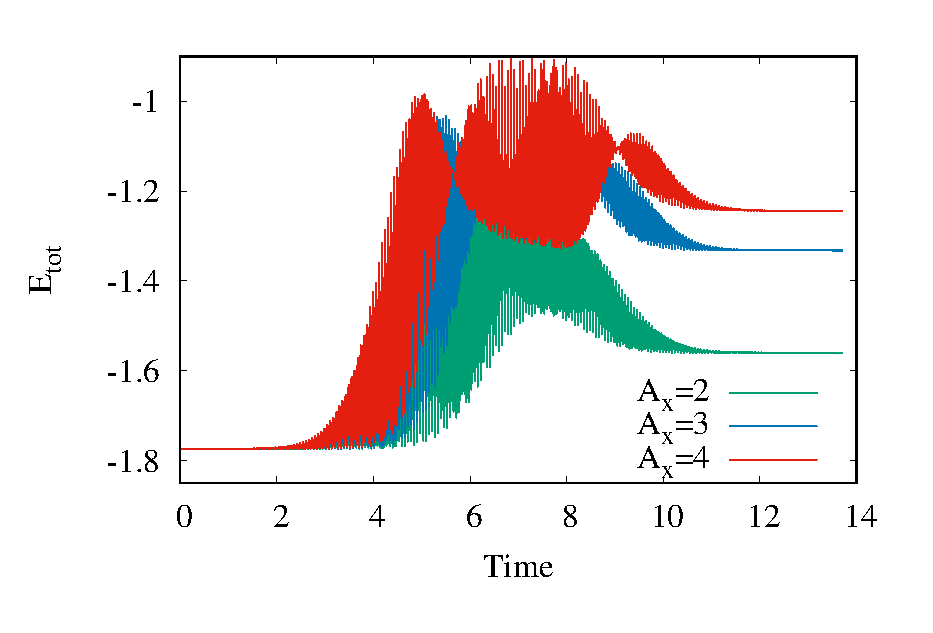
\includegraphics[width=1\linewidth]{Chapters/Fermi_surface/figures/appendix/dEtot_time_xray.eps}} (b) \\
\end{minipage}
\caption{Total energy of the system as function on time in case of $U=2$ for different pulse frequencies: (a) $\omega=1.4$; (b) $\omega=50$.}
\label{fig:E_tot_time_FS}
\end{figure}

Double occupancy decreases in the case of $\omega=1.4$ (Fig.~\ref{fig:docc_time_FS}a) and increases for $\omega=50$ (Fig.~\ref{fig:docc_time_FS}b).
\begin{figure}[h!]
\begin{minipage}[h]{0.5\linewidth}
\center{\includegraphics[width=1\linewidth]{Chapters/Fermi_surface/figures/appendix/docc_e_IR.eps}} (a) \\
\end{minipage}
\hfill
\begin{minipage}[h]{0.5\linewidth}
\center{\includegraphics[width=1\linewidth]{Chapters/Fermi_surface/figures/appendix/docc_e_xray.eps}} (b) \\
\end{minipage}
\caption{Double occupancy of the system as function on time in case of $U=2$ for different pulse frequencies: (a) $\omega=1.4$; (b) $\omega=50$.}
\label{fig:docc_time_FS}
\end{figure}

The difference between the initial and final values of the total energy $\bigtriangleup E_{tot}=E_{initial}-E_{final}$ displays absorption for systems with different interactions. The Fig.~\ref{fig:dEtot_A_FS} shows the dependence of $\bigtriangleup E_{tot}$ on the magnitude of the maximum projection of the vector potential $A_x$. The nonlinear dynamics of adsorption with increasing Coulomb interaction is visible.
\begin{figure}[h!]
\begin{minipage}[h]{0.5\linewidth}
\center{\includegraphics[width=1\linewidth]{Chapters/Fermi_surface/figures/appendix/dEtot_IR_s_Evg.eps}} (a) \\
\end{minipage}
\hfill
\begin{minipage}[h]{0.5\linewidth}
\center{\includegraphics[width=1\linewidth]{Chapters/Fermi_surface/figures/appendix/dEtot_xray.eps}} (b) \\
\end{minipage}
\caption{Difference between the initial and final values of the total energy $\bigtriangleup E_{tot}=E_{initial}-E_{final}$ as function on $A_x$: (a) $\omega=1.4$; (b) $\omega=50$.}
\label{fig:dEtot_A_FS}
\end{figure}


\begin{figure}[h!]
\begin{minipage}[h]{0.5\linewidth}
\center{\includegraphics[width=1\linewidth]{Chapters/Fermi_surface/figures/appendix/dEpot_IR_Evg.eps}} (a) \\
\end{minipage}
\hfill
\begin{minipage}[h]{0.5\linewidth}
\center{\includegraphics[width=1\linewidth]{Chapters/Fermi_surface/figures/appendix/dEpot_xray_Evg.eps}} (b) \\
\end{minipage}
\caption{Difference between the initial and final values of the kinetic and potential energies as function on $A_x$: (a) $\omega=1.4$; (b) $\omega=50$.}
\label{fig:dEpot_A_FS}
\end{figure}

Contributions of potential and kinetic energy to absorption are shown in Fig.~\ref{fig:dEpot_A_FS}.